see Roe theorem \cite[p.417]{Toro}
\subsection{Convergence analysis}
\subsection{One-dimensional stability analysis}
A stability analysis of the one-dimensional DGMPM scheme is performed on a scalar linear hyperbolic equation. Following \cite{Hirsch}, the discretized equation is written in a finite difference sense in order to perform a von Neumann linear stability analysis.
\subsubsection*{Model equation - Space discretization}
We consider the scalar linear advection equation for an arbitrary quantity $q=\rho \bar{q}$ moving at the constant speed $a \in \Rbb^{+*}$ in a homogeneous one-dimensional medium of length $l$:
\begin{equation}
\drond{\bar{q}}{t} + a\drond{\bar{q}}{X} = 0 \label{eq:scalar_advection}
\end{equation}
The specific flux function is $\bar{\Fc} = a\bar{q}$ and equation \eqref{eq:scalar_advection} is discretized with the discontinuous Galerkin material point method. Thus, it is assumed that the medium has been divided with $P$ material points arbitrarily distributed in $E$ two-nodes elements of constant length $\Delta X$ (figure~\ref{fig:1Dmesh}). The grid mesh is such that at least one particle lies in every cell during the computation in order to ensure that there is no hole in the bar. Moreover, periodic boundary conditions are considered to simplify the analysis.
\begin{figure}[h!]
  \centering
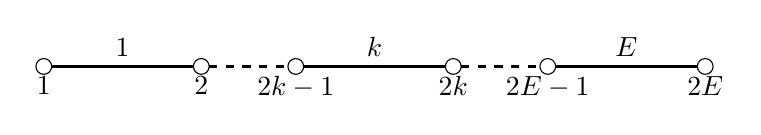
\begin{tikzpicture}
  \draw (2.3,0) circle (0.1) node [below] {$1$};
  \draw (4.3,0) circle (0.1) node [below] {$2$};
  \draw[thick] (2.4,0) -- (4.2,0) node [above,midway] {$1$};
  \draw[thick,dashed] (4.4,0) -- (5.4,0);
  \draw (5.5,0) circle (0.1) node [below] {$2k-1$};
  \draw (7.5,0) circle (0.1) node [below] {$2k$};
  \draw[thick] (5.6,0) -- (7.4,0) node [above,midway] {$k$};
  \draw[thick,dashed] (7.6,0) -- (8.6,0);
  \draw (8.7,0) circle (0.1) node [below] {$2E-1$};
  \draw (10.7,0) circle (0.1) node [below] {$2E$};
  \draw[thick] (8.8,0) -- (10.6,0) node [above,midway] {$E$};
\end{tikzpicture}

  \caption{One-dimensional mesh made of $E$ elements of constant length $\Delta X = \frac{l}{E}$.}\label{fig:1Dmesh}
\end{figure}

Since fields are carried by particles, we seek for the scheme equation that gives the solution $\bar{Q}^{n+1}_\alpha$ at material point $\alpha$ and time step $n+1$, with respect to the solutions of other particles at previous time step.
In this section, Latin and Greek indices denote respectively nodes and material points, $S_{i\alpha}$ is thus the shape function of node $i$ evaluated at the position of material points $\alpha$. Linear shape functions defined in element $k$ yield:
\begin{equation}
S_{2k-1}(X)= \frac{X_{2k} - X}{\Delta X} \qquad S_{2k}(X)= \frac{X -X_{2k-1}}{\Delta X} \qquad X \in \[X_{2k-1},X_{2k}\]
\end{equation}
Furthermore, the cell containing a given particle $\beta$ will be denoted by $c(\beta)$ and this notation will be also used for nodes, for instance: $c(2k-1)=c(2k)=k$.
\subsubsection*{DGMPM scheme equation}
The method followed to write the scheme equation is to trace backward the numerical procedure described in section \ref{sec:DGMPM} in order to get an expression for material point $\alpha$:
\begin{equation}
\bar{Q}^{n+1}_\alpha = f\(\bar{Q}^{n}_\mu\) \qquad  \mu=1,..,P
\end{equation} 
where $f$ is a function representing the DGMPM scheme.
Quantities at time $t^{n+1}$ are obtained by interpolating nodal solutions of the discrete equation \eqref{eq:DGMPM_discrete} thanks to mapping \eqref{eq:DGMPM_node2points}: 
\begin{equation}
\bar{Q}^{n+1}_\alpha = \sum_{i=1}^{E}  \( S_{2i-1,\alpha}\bar{q}_{2i-1}^{n+1} + S_{2i,\alpha}\bar{q}_{2i}^{n+1}\) \label{eq:stab_node2points}
\end{equation}
Interfaces fluxes are $\Fc_N =  (aq^*) N$, where $q^*$ is the stationary solution of Riemann problem at cell interface and $N=\pm 1$ the outward unit normal. Nodal solutions at time $n+1$ in equation \eqref{eq:stab_node2points} are the result of the discrete system \eqref{eq:DGMPM_discrete}:
\begin{equation}
\bar{q}^{n+1}_{i}  =\bar{q}^{n}_{i} + \frac{\Delta t}{M^L_{i}} a \( \sum_{j=1}^{2E} K_{i,j} \bar{q}^n_{j} - q^*_{i}N_i \) \quad \text{(no sum on $i$)} \label{eq:stab_discrete}
\end{equation}
Provided linear shape functions, the lumped mass and the pseudo-stiffness matrices are:
\begin{align}
&M^L_i = \sum_{\beta=1}^{P} S_{i\beta} m_\beta \\
& K_{2i-1,j} = \sum_{\lambda=1}^{P} \drond{S_{2i-1,\lambda}}{X} m_\lambda S_{j\lambda} = -\sum_{\lambda=1}^{P} \frac{m_\lambda S_{j\lambda}}{\Delta X} \\
& K_{2i,j} =
  \sum_{\lambda=1}^{P} \drond{S_{2i,\lambda}}{X} m_\lambda S_{j\lambda} = \sum_{\lambda=1}^{P} \frac{m_\lambda S_{j\lambda}}{\Delta X} 
\end{align}
where $m_\alpha$ is the mass of $\alpha^{\text{th}}$ material point. Since the pseudo-stiffness matrix component $K_{ij}$ is zero if $i$ and $j$ are not connected by an element, due to the discontinuities of shape functions, the sum over $j$ in equation \eqref{eq:stab_discrete} reduces to: $\sum_{j=1}^{2E} K_{2i-1,j} \bar{q}^n_{j} =  K_{2i-1,2i-1} \bar{q}^n_{2i-1} + K_{2i-1,2i} \bar{q}^n_{2i}$ . We can thus write:
\begin{equation}
\frac{\sum_{j} K_{2i-1,j}}{M^L_{2i-1}}\bar{q}^n_{j} = 
- \frac{\sum_{\lambda}^{} \(S_{2i-1,\lambda}\bar{q}^n_{2i-1} + S_{2i,\lambda}\bar{q}^n_{2i} \)}{\Delta X\sum_{\beta} S_{2i-1,\beta}}  \qquad ; \qquad \frac{\sum_{j} K_{2i,j}}{M^L_{2i}}\bar{q}^n_{j} =  \frac{ \sum_{\lambda}^{} \(S_{2i-1,\lambda}\bar{q}^n_{2i-1} + S_{2i,\lambda}\bar{q}^n_{2i}\)}{\Delta X\sum_{\beta} S_{2i,\beta}}  \label{eq:stab_volumic_fluxes}
\end{equation}
Since waves travel from left to right ($a>0$), the stationary solution is equal to $q_L$ on an interface, that is:
\begin{align}
& q_{2i-1}^* = \rho \bar{q}^n_{2i-2} \quad ; \quad q_{2i}^* = \rho \bar{q}^n_{2i} \\
&N_{2i-1} = -1 \quad ; \quad N_{2i} = 1
\end{align} 
Moreover, in a homogeneous medium the mass density can be replaced by $\rho = N^{c( \alpha)} m_\alpha/\Delta X$ where $N^{c( \alpha)}$ is the number of particles in the cell that contains the $\alpha^{th}$ material point. Then, we have:
\begin{equation}
\frac{q_{2i-1}^*}{M_{2i-1}^L} = \frac{N^{c( \alpha)}}{\Delta X \sum_\beta S_{2i-1,\beta}} \bar{q}^n_{2i-2}  \quad ; \quad \frac{q_{2i}^*}{M_{2i}^L} = \frac{N^{c( \alpha)}}{\Delta X \sum_\beta S_{2i,\beta}} \bar{q}^n_{2i} \label{eq:stab_interface_fluxes}
\end{equation}
Equations \eqref{eq:stab_volumic_fluxes} and \eqref{eq:stab_interface_fluxes} are introduced into discrete system \eqref{eq:stab_discrete} so that equation \eqref{eq:stab_node2points} is rewritten as:
\begin{equation} 
\begin{aligned}
\bar{Q}^{n+1}_\alpha =  \sum_{i=1}^{2E} S_{i\alpha}\bar{q}^n_{i} + &  a\frac{\Delta t}{\Delta X} \sum_{i=1}^{E}  \sum_{\lambda=1}^{P}\( S_{2i-1,\lambda}\bar{q}^n_{2i-1} + S_{2i,\lambda}\bar{q}^n_{2i}\) \[ \frac{S_{2i,\alpha} }{\sum_{\beta} S_{2i,\beta}}   - \frac{S_{2i-1,\alpha} }{\sum_{\beta} S_{2i-1,\beta}} \] \\
+& a\frac{\Delta t}{\Delta X} N^{c( \alpha)} \sum_{i=1}^{E} \[ \frac{S_{2i-1,\alpha}}{\sum_\beta S_{2i-1,\beta}} \bar{q}^n_{2i-2} - \frac{S_{2i,\alpha} }{\sum_\beta S_{2i,\beta}} \bar{q}^n_{2i}\]   
\end{aligned}\label{eq:stab_before_mapping}
\end{equation} 
In equation \eqref{eq:stab_before_mapping} the solutions at nodes result from the convection step \eqref{eq:DGMPM_points2nodes}:
\begin{equation}
\bar{q}^{n}_{i} = \frac{\sum_\mu S_{i\mu}m_\mu \bar{Q}^n_{\mu}}{\sum_\gamma S_{i\gamma}m_\gamma} = \frac{\sum_\mu S_{i\mu} \bar{Q}^n_{\mu}}{\sum_\gamma S_{i\gamma}} \label{eq:stab_mapping}
\end{equation}
Thus, introduction of mapping \eqref{eq:stab_mapping} in equation \eqref{eq:stab_before_mapping} and permutation of sums over $\mu$ and $i$ lead after some simplifications to the scheme equation:
\begin{equation} 
\begin{aligned}
\bar{Q}^{n+1}_\alpha = \sum_{\mu=1}^{P} \bar{Q}^n_{\mu} \left\lbrace \sum_{i=1}^{2E} S_{i\alpha}\frac{S_{i\mu}}{\sum_\gamma S_{i\gamma}} + \right. &  a\frac{\Delta t}{\Delta X} \sum_{i=1}^{E}  \( S_{2i-1,\mu} +S_{2i,\mu}\) \[ \frac{S_{2i,\alpha} }{\sum_{\beta} S_{2i,\beta}}   - \frac{S_{2i-1,\alpha} }{\sum_{\beta} S_{2i-1,\beta}} \]  \\ + &  \left. a\frac{\Delta t}{\Delta X} N^{c( \alpha)} \sum_{i=1}^{E} \[ \frac{S_{2i-1,\alpha}}{\sum_\beta S_{2i-1,\beta}} \frac{S_{2i-2,\mu}}{\sum_\gamma S_{2i-2,\gamma}} - \frac{S_{2i,\alpha} }{\sum_\beta S_{2i,\beta}} \frac{S_{2i,\mu}}{\sum_\gamma S_{2i,\gamma}}\]\right\rbrace
\end{aligned}
\end{equation}
This recurrence relation can be further simplified by viewing that the term in parentheses is non zero and equal to one, due to partition of unity, only for element $i=c( \mu)$. On the other hand, $S_{2i-1,\alpha}S_{2i-2,\mu}$ is non zero only if cell $i$ contains material point $\alpha$ and is such that $i=c(\mu)+1$. Hence, the scheme equation reads:
\begin{equation} 
\begin{aligned}
\bar{Q}^{n+1}_\alpha = \sum_{\mu=1}^{P} \bar{Q}^n_{\mu} \left\lbrace \sum_{i=1}^{2E} S_{i\alpha}\frac{S_{i\mu}}{\sum_\gamma S_{i\gamma}} + \right. &  a\frac{\Delta t}{\Delta X}  \[ \frac{S_{2c(\mu),\alpha} }{\sum_{\beta} S_{2c(\mu),\beta}}   - \frac{S_{2c(\mu)-1,\alpha} }{\sum_{\beta} S_{2c(\mu)-1,\beta}} \]  \\ + &  \left. a\frac{\Delta t}{\Delta X} N^{c(\alpha)} \[ \frac{S_{2c(\mu)+1,\alpha}}{\sum_\beta S_{2c(\mu)+1,\beta}} \frac{S_{2c(\mu),\mu}}{\sum_\gamma S_{2c(\mu),\gamma}} - \frac{S_{2c(\mu),\alpha}S_{2c(\mu),\mu} }{(\sum_\beta S_{2c(\mu),\beta})^2} \]\right\rbrace \label{eq:Dalpha_mu}
\end{aligned}
\end{equation}
which can be written for simplicity:
\begin{equation}
\bar{Q}^{n+1}_\alpha = \sum_{\mu=1}^P \bar{Q}^n_{\mu} D_{\alpha\mu} \label{eq:scheme_Dpi}
\end{equation}
The numerical solution $\bar{Q}^{n+1}_\alpha$ depends on the Courant number $a\Delta t / \Delta X$ and on the position of material points within the grid mesh through the shape functions in the expression of coefficients $D_{\alpha\mu}$. Furthermore, the first (\textit{resp. second}) brackets in equation \eqref{eq:Dalpha_mu} involve shape functions that are non zero if material point $\mu$ and $\alpha$ lie in the same cell (\textit{resp. previous cell}). This property means that the numerical domain of dependence of the DGMPM for scalar linear advection with $a>0$ covers two cells regardless of the number of material points.

\subsubsection*{The von Neumann linear stability analysis}
The computational domain is now repeated periodically by mapping it to the domain $[-l,0]$ so that the solution at material point $\beta$ and time step $n$ is expanded into a discrete Fourier basis of $2E+1$ harmonics over the domain $X \in \[-l,l\]$:
\begin{equation}
\bar{Q}^{n}_\beta = \sum_{j=-E}^{E}A_j^n e^{I \beta k_j \Delta X}
\end{equation}
with $A^n_j$, the magnitude of the $j^\text{th}$ harmonic at time step $n$, $I = \sqrt{-1}$, and $k_j$ a wave number. Introduction of this expansion in equation \eqref{eq:scheme_Dpi} yields:
\begin{equation}
A_j^{n+1} e^{I \alpha k_j \Delta X} = \sum_{\mu=1}^P A_j^n D_{\alpha\mu}e^{I \mu k_j \Delta X}\quad \forall j=-E,...,E
\end{equation}
The amplification factor between two time steps at a given point is defined as:
\begin{equation}
\frac{A_j^{n+1}}{A_j^n} = \sum_{\mu=1}^P e^{I (\mu -\alpha)k_j \Delta X} D_{\alpha\mu} \quad \forall j=-E,...,E \label{eq:fourier}
\end{equation}
A necessary condition to ensure the stability of a numerical scheme is that the amplification factor must be lower than one in modulus: $\abs{A^{n+1}/A^n} < 1$. This upper bound allows to ensure that eventual errors do not increase during the computation. For expression \eqref{eq:fourier}, this leads to:
\begin{equation}
 \abs{\sum_{\mu=1}^P e^{I (\mu -\alpha)k_j \Delta X} D_{\alpha\mu}} \leq \sum_{\mu=1}^P \abs{e^{I (\mu -\alpha)k_j \Delta X} D_{\alpha\mu}} = \sum_{\mu=1}^P \abs{D_{\alpha\mu}}
\end{equation}
where the triangle inequality, and the unit modulus of the complex number $e^{I (\mu -\alpha)k_j \Delta X}$ have been used.
Hence, the DGMPM scheme is stable for a given discretization if the Courant number is set so that the following condition is satisfied:
\begin{equation}
\sum_{\mu=1}^P \abs{D_{\alpha\mu}} \leq 1 \label{eq:stability}
\end{equation}
According to the scheme equation \eqref{eq:Dalpha_mu}, such a stability condition can be very hard to deal with analytically for general discretizations. However, the particular configuration for which one single particle lies in each cell can be studied analytically. In this case, condition \eqref{eq:stability} reads:
\begin{equation}
\sum_{\mu=1}^P \abs{D_{\alpha\mu}} = \abs{1 - a\frac{\Delta t}{\Delta X} } +  \abs{ a\frac{\Delta t}{\Delta X} } \leq 1 \label{eq:1ppc_stab}
\end{equation}
which is satisfied for all $a\frac{\Delta t}{\Delta X} \leq 1$ regardless of the positions of particles.
Hence, this space discretization leads to a stable scheme for the optimal Courant condition while the classical DGFEM scheme developed in \cite{Chavent_Salzano} is restricted to condition $\Delta t / \Delta X = \Oc(\sqrt{\Delta X})$. Recall that this DGMPM space discretization can be viewed as a DGFEM with reduced integration of the weak form (see section \ref{section:discretization}). Hence, combination of reduced integration with projections between mesh nodes and integration points allows to improve the restrictive stability condition of original DGFEM \cite{Chavent_Salzano,NeutronDG}. However, this optimal condition is no longer valid for discretizations involving more than one material point per cell. Indeed, figure \ref{figure:Amplification_factor} shows the evolution of the amplification factor with respect to the Courant number for several (regular) discretizations. Since the scheme equation \eqref{Dalpha_mu} depends on the particle considered, those curves are plotted for each material point contained in a given cell. In figures \ref{figure:Amplification_factor}\subref{subfig:CFL_2ppc} and \ref{figure:Amplification_factor}\subref{subfig:CFL_3ppc} we can see that the amplification factor satisfies the stability condition \eqref{stability} for CFL numbers lower than one.

%%% Table of CFL that can be reached depending on the discretization
Two material points in each cell are considered in figure \ref{figure:Amplification_factor}\subref{subfig:CFL_2ppc}, with either a symmetrical or an offset configuration, respectively shown in figures \ref{figure:Amplification_factor}\subref{subfig:conf1} and \ref{figure:Amplification_factor}\subref{subfig:conf2}. It also appears that the more restrictive condition on CFL number is given by the upwind (first) material point ($CFL=0.43$ for symmetrical configuration and $CFL=0.34$ for shifted one). Moreover, the material points positions influence the stability condition as shown by the shifted configuration for which the result is more restrictive. Similar observations can be made with figure \ref{figure:Amplification_factor}\subref{subfig:CFL_3ppc} in which three particles are considered. In that case, Courant number decreases to $CFL=0.29$ for configuration \ref{figure:Amplification_factor}\subref{subfig:conf3} and $CFL=0.26$ for configuration \ref{figure:Amplification_factor}\subref{subfig:conf4}. 

The von Neumann linear stability analysis performed in this section provides an explicit (nonlinear) condition \eqref{stability} that must be satisfied in order to ensure the stability of the DGMPM scheme. First, this relation allows to fully exploit the ability of the method to rebuild the grid mesh arbitrarily. Indeed, after such a procedure, the number and positions of material points in grid cells can change and one must be able to adapt properly the CFL number in order to ensure stability. An advantage on the original MPM is hence highlighted since no stability condition exists for the latter scheme. Second, it has been shown that some DGMPM discretizations provide an improvement of the restrictive CFL number that applies to the DGFEM scheme. In particular, the optimal condition allowing to capture discontinuities ($CFL=1$) can be reached when one particle lies in each cell of the grid mesh. This property turns out to be a strength for the DGMPM since it aims at follow waves accurately as shown with the following numerical results.


+ RK2 ??
\subsection{Two-dimensional stability analysis}



%%% Local Variables: 
%%% mode: latex
%%% TeX-master: "../mainManuscript"
%%% End:
